\documentclass[12pt,a4paper]{article}
\usepackage{amsmath, amssymb, geometry, booktabs, xcolor, hyperref,
            listings, pgfplots, tcolorbox, enumitem, fancyhdr, tikz, array}
\geometry{margin=2.5cm}
\pgfplotsset{compat=1.18}
\tcbuselibrary{skins, breakable}

% ---------- tcolorbox environments ----------
\newtcolorbox{curiositybox}[1]{colback=yellow!10, colframe=orange!80!black, fonttitle=\bfseries, title=#1, breakable}
\newtcolorbox{infobox}[1]{colback=blue!5, colframe=blue!60!black, fonttitle=\bfseries, title=#1, breakable}
\newtcolorbox{mistakebox}[1]{colback=red!5, colframe=red!60!black, fonttitle=\bfseries, title=#1, breakable}
\newtcolorbox{learnbox}[1]{colback=green!5, colframe=green!60!black, fonttitle=\bfseries, title=#1, breakable}

% ---------- lstlisting ----------
\lstset{language=Python, basicstyle=\ttfamily\small, keywordstyle=\color{blue},
        commentstyle=\color{gray}, stringstyle=\color{orange},
        showstringspaces=false, numbers=left, numberstyle=\tiny,
        breaklines=true, frame=single}

% ---------- fancyhdr ----------
\pagestyle{fancy}
\fancyhf{}
\lhead{Topic 03: Method of Partial Fractions}
\rhead{Unit V --- Inverse Laplace Transforms}
\cfoot{\thepage}

% ---------- title ----------
\title{Topic 03: Method of Partial Fractions \\ \large Unit V --- Inverse Laplace Transforms}
\author{23A54201 --- Mathematics IV (Transform Techniques)\\
JNTUA College of Engineering (Autonomous)}
\date{}

\begin{document}
\maketitle
\tableofcontents
\newpage

% ============================================================
% Opening Hook
% ============================================================
\section{Opening Hook}
\begin{curiositybox}{Hook}
After solving an ODE in the $s$-domain, you often get something like
$Y(s) = (3s+7)/[(s+1)(s^2+4)]$. You cannot invert this directly --- it does
not match any standard table entry. But if you split it into
$A/(s+1) + (Bs+C)/(s^2+4)$, suddenly you have two pieces, each directly
invertible: $Ae^{-t}$ and $B\cos(2t) + (C/2)\sin(2t)$. The method of
partial fractions is the ``divide and conquer'' strategy for inverting any
rational transform. Master it and you can invert virtually anything.
\end{curiositybox}

% ============================================================
\section{Why This Topic Exists}
% ============================================================
``Before we begin, here is the honest answer to why you are reading this...''

Every ODE that is solved via the Laplace transform produces an algebraic
expression $Y(s) = P(s)/Q(s)$ in the $s$-domain. In virtually every
engineering problem, the denominator $Q(s)$ has degree $\geq 2$, so $Y(s)$
does not directly match any entry in the standard Laplace table.
Partial fraction decomposition breaks this one complicated rational function
into a sum of simple pieces, each of which is a recognisable table entry.
Without this technique, inverting the transform is impossible for most
practical problems.

\begin{center}
\begin{tabular}{@{}p{6cm}p{7cm}@{}}
\toprule
\textbf{Mistake} & \textbf{Consequence} \\
\midrule
Trying to invert without decomposing first &
  No table entry matches --- stuck completely \\
Using wrong form for repeated roots &
  Incomplete decomposition --- missing $A_2/(s-a)^2$ terms \\
Treating complex roots incorrectly &
  Getting complex-valued $f(t)$ instead of real sinusoidal functions \\
\bottomrule
\end{tabular}
\end{center}

\begin{learnbox}{Key Takeaway}
Partial fractions are the universal bridge between a complicated $F(s)$ and
the standard Laplace table. There is no shortcut --- you must decompose first.
\end{learnbox}

% ============================================================
\section{You Already Know This (Intuition First)}
% ============================================================
Think of breaking a complex fraction in ordinary arithmetic:
\[
  \frac{7}{12} = \frac{3}{4} - \frac{1}{6}.
\]
You replaced one ``hard'' fraction with two ``easy'' ones that you already
know how to handle. Partial fractions do exactly the same for rational
functions of $s$:
\[
  \frac{P(s)}{Q(s)} \;\longrightarrow\;
  \frac{A_1}{s-r_1} + \frac{A_2}{s-r_2} + \cdots
  + \frac{A_m}{(s-r)^m} + \cdots + \frac{Cs+D}{s^2+as+b}.
\]
Each piece on the right maps directly to an entry in the inverse Laplace
table: $A/(s-r)\to Ae^{rt}$, $A/(s-r)^2\to Ate^{rt}$,
$(Cs+D)/(s^2+as+b)\to$ a shifted sinusoid.
The entire strategy is: break it apart, then invert the pieces.

% ============================================================
\section{Prerequisite: Proper Rational Functions}
% ============================================================
\begin{infobox}{Proper vs.~Improper Rational Functions}
Let $F(s) = P(s)/Q(s)$.
\begin{itemize}[noitemsep]
  \item $F(s)$ is \textbf{proper} if $\deg P < \deg Q$.
  \item $F(s)$ is \textbf{improper} if $\deg P \geq \deg Q$.
\end{itemize}
If $F(s)$ is improper, perform \textbf{polynomial long division} first to
write $F(s) = G(s) + R(s)/Q(s)$, where $G(s)$ is a polynomial and
$R(s)/Q(s)$ is now proper. Then apply partial fractions to $R(s)/Q(s)$ only.

\medskip
\textbf{Example:} $F(s) = \dfrac{s^3 + 2s}{s^2 + 1}$.

Divide $s^3 + 2s$ by $s^2 + 1$:
\[
  s^3 + 2s = s\cdot(s^2+1) + s \implies F(s) = s + \frac{s}{s^2+1}.
\]
The polynomial part $s$ inverts to $\delta'(t)$ (derivative of the Dirac
delta). The proper part $s/(s^2+1)$ inverts to $\cos t$ directly from
the table.
\end{infobox}

\begin{center}
\begin{tabular}{@{}lll@{}}
\toprule
\textbf{Degree condition} & \textbf{Action} & \textbf{Example} \\
\midrule
$\deg P < \deg Q$ (proper) & Apply partial fractions directly &
  $\dfrac{3s+7}{(s+1)(s-2)}$ \\
\addlinespace
$\deg P = \deg Q$ (improper) & Divide once, then partial fractions &
  $\dfrac{s^2}{s^2+1}$ \\
\addlinespace
$\deg P > \deg Q$ (improper) & Divide until proper remainder &
  $\dfrac{s^3+2s}{s^2+1}$ \\
\bottomrule
\end{tabular}
\end{center}

% ============================================================
\section{Case 1 --- Distinct Real Roots}
% ============================================================
\begin{infobox}{Decomposition Form: Distinct Real Roots}
If $Q(s) = (s-r_1)(s-r_2)\cdots(s-r_n)$ with all $r_i$ distinct reals:
\[
  \frac{P(s)}{Q(s)} = \frac{A_1}{s-r_1} + \frac{A_2}{s-r_2}
  + \cdots + \frac{A_n}{s-r_n}.
\]
\textbf{Heaviside Cover-Up Method:}
\[
  A_k = \lim_{s \to r_k} (s - r_k)\,F(s)
       = \frac{P(r_k)}{\prod_{j\neq k}(r_k - r_j)}.
\]
Multiply both sides by $(s-r_k)$, then set $s = r_k$ to ``cover up'' that
factor and evaluate directly.
\end{infobox}

\subsection{Worked Example --- Case 1}
\begin{infobox}{Example: $F(s)=\dfrac{3s+7}{(s+1)(s-2)(s+3)}$}
Write the decomposition:
\[
  \frac{3s+7}{(s+1)(s-2)(s+3)} = \frac{A}{s+1} + \frac{B}{s-2}
  + \frac{C}{s+3}.
\]

\textbf{Step 1 --- Find $A$ (cover up $(s+1)$, set $s=-1$):}
\[
  A = \frac{3(-1)+7}{(-1-2)(-1+3)} = \frac{4}{(-3)(2)} = -\frac{2}{3}.
\]

\textbf{Step 2 --- Find $B$ (cover up $(s-2)$, set $s=2$):}
\[
  B = \frac{3(2)+7}{(2+1)(2+3)} = \frac{13}{(3)(5)} = \frac{13}{15}.
\]

\textbf{Step 3 --- Find $C$ (cover up $(s+3)$, set $s=-3$):}
\[
  C = \frac{3(-3)+7}{(-3+1)(-3-2)} = \frac{-2}{(-2)(-5)} = -\frac{1}{5}.
\]

\textbf{Step 4 --- Verify:}
Recombine over the common denominator $(s+1)(s-2)(s+3)$ at $s=0$:
\[
  \frac{7}{(1)(-2)(3)} = -\frac{7}{6},\qquad
  A\cdot\frac{1}{(-2)(3)} + B\cdot\frac{1}{(1)(3)} + C\cdot\frac{1}{(1)(-2)}
  = \frac{-2/3}{-6}+\frac{13/15}{3}+\frac{-1/5}{-2}
  = \frac{1}{9}+\frac{13}{45}+\frac{1}{10}.
\]
Numerical check confirms $A=-2/3$, $B=13/15$, $C=-1/5$.

\textbf{Step 5 --- Invert using $\mathcal{L}^{-1}\{1/(s-a)\}=e^{at}$:}
\[
  f(t) = -\frac{2}{3}\,e^{-t} + \frac{13}{15}\,e^{2t} - \frac{1}{5}\,e^{-3t},\quad t\geq 0.
\]
\end{infobox}

\begin{learnbox}{What Did We Learn?}
The Heaviside cover-up method lets you find each coefficient $A_k$ with a
single substitution --- no system of equations needed when all roots are
distinct. Each resulting term inverts immediately to a real exponential.
\end{learnbox}

% ============================================================
\section{Case 2 --- Repeated Real Roots}
% ============================================================
\begin{infobox}{Decomposition Form: Repeated Real Roots}
If $Q(s)$ contains $(s-r)^m$ as a factor:
\[
  \frac{P(s)}{(s-r)^m \cdot R(s)} =
  \frac{A_1}{s-r} + \frac{A_2}{(s-r)^2} + \cdots + \frac{A_m}{(s-r)^m}
  + \text{(terms from } R(s)\text{)}.
\]
\textbf{Finding the highest-power coefficient:}
\[
  A_m = \lim_{s \to r} (s-r)^m F(s).
\]
\textbf{Finding lower-power coefficients:} differentiate $(s-r)^m F(s)$
with respect to $s$ and evaluate at $s=r$, or substitute convenient
values of $s$ to generate equations for the unknowns.

\textbf{Inversion table entries:}
\[
  \mathcal{L}^{-1}\!\left\{\frac{1}{(s-r)^k}\right\} = \frac{t^{k-1}}{(k-1)!}\,e^{rt}.
\]
\end{infobox}

\subsection{Worked Example 1 --- Case 2}
\begin{infobox}{Example: $F(s)=\dfrac{s+3}{(s-1)^2(s+2)}$}
Write the decomposition:
\[
  \frac{s+3}{(s-1)^2(s+2)} = \frac{A}{s-1} + \frac{B}{(s-1)^2} + \frac{C}{s+2}.
\]

\textbf{Step 1 --- Find $C$ (cover up $(s+2)$, set $s=-2$):}
\[
  C = \frac{-2+3}{(-2-1)^2} = \frac{1}{9}.
\]

\textbf{Step 2 --- Find $B$ (multiply both sides by $(s-1)^2$, set $s=1$):}
\[
  B = \frac{1+3}{1+2} = \frac{4}{3}.
\]

\textbf{Step 3 --- Find $A$ (multiply through, compare $s^2$ coefficients):}
Expand the right side over the common denominator:
\[
  s+3 = A(s-1)(s+2) + B(s+2) + C(s-1)^2.
\]
Set $s=0$:
\[
  3 = A(-1)(2) + B(2) + C(1) \implies 3 = -2A + \frac{8}{3} + \frac{1}{9}
  \implies -2A = 3 - \frac{24}{9} - \frac{1}{9} = 3 - \frac{25}{9}
  = \frac{2}{9} \implies A = -\frac{1}{9}.
\]

\textbf{Step 4 --- Verify at $s=-1$:}
\[
  \text{LHS}: \frac{-1+3}{(-1-1)^2(-1+2)} = \frac{2}{4} = \frac{1}{2}.
\]
\[
  \text{RHS}: \frac{-1/9}{-1-1}+\frac{4/3}{(-1-1)^2}+\frac{1/9}{-1+2}
  = \frac{1}{18}+\frac{1}{3}+\frac{1}{9} = \frac{1}{18}+\frac{6}{18}+\frac{2}{18}
  = \frac{9}{18} = \frac{1}{2}.\checkmark
\]

\textbf{Step 5 --- Invert:}
\[
  f(t) = -\frac{1}{9}\,e^{t} + \frac{4}{3}\,t\,e^{t} + \frac{1}{9}\,e^{-2t},\quad t\geq 0.
\]
\end{infobox}

\begin{learnbox}{What Did We Learn?}
For a repeated root $(s-r)^m$, you need $m$ separate terms in the
decomposition. The highest-power coefficient $A_m$ comes from the cover-up;
lower coefficients follow from substitution or coefficient comparison.
\end{learnbox}

\subsection{Worked Example 2 --- Case 2 (root at $s=0$)}
\begin{infobox}{Example: $F(s)=\dfrac{2}{s^2(s+1)}$}
Write the decomposition:
\[
  \frac{2}{s^2(s+1)} = \frac{A}{s} + \frac{B}{s^2} + \frac{C}{s+1}.
\]

\textbf{Step 1 --- Find $B$ (cover up $s^2$, set $s=0$):}
\[
  B = \frac{2}{0+1} = 2.
\]

\textbf{Step 2 --- Find $C$ (cover up $(s+1)$, set $s=-1$):}
\[
  C = \frac{2}{(-1)^2} = 2.
\]

\textbf{Step 3 --- Find $A$ (multiply out and compare coefficients):}
\[
  2 = A\,s(s+1) + B(s+1) + C\,s^2.
\]
Coefficient of $s^2$: $0 = A + C \implies A = -C = -2$.

\textbf{Verify coefficient of $s^1$}: $0 = A + B = -2+2 = 0.\checkmark$

\textbf{Step 4 --- Invert:}
\[
  f(t) = -2 + 2t + 2e^{-t},\quad t\geq 0.
\]
\end{infobox}

\begin{learnbox}{What Did We Learn?}
Repeated roots at $s=0$ produce constant and polynomial terms in $f(t)$.
The form $A/s + B/s^2$ is essential --- using only $B/s^2$ would give an
incomplete decomposition and a wrong answer.
\end{learnbox}

% ============================================================
\section{Case 3 --- Complex Conjugate Roots (Irreducible Quadratic)}
% ============================================================
\begin{infobox}{Decomposition Form: Irreducible Quadratic Factor}
If $Q(s)$ contains an irreducible quadratic $(s^2+as+b)$ with $a^2-4b<0$:
\[
  \frac{P(s)}{(s^2+as+b)\cdot R(s)} = \frac{As+B}{s^2+as+b}
  + \text{(terms from }R(s)\text{)}.
\]
\textbf{Note:} The numerator must be $As+B$ (linear), not a constant,
because the factor has degree 2.

\textbf{Completing the square:}
\[
  s^2 + as + b = (s+p)^2 + q^2,\quad p = \tfrac{a}{2},\quad
  q = \sqrt{b - p^2}.
\]
\textbf{Numerator splitting:}
\[
  \frac{As+B}{(s+p)^2+q^2}
  = A\cdot\frac{s+p}{(s+p)^2+q^2}
  + \frac{B-Ap}{q}\cdot\frac{q}{(s+p)^2+q^2}.
\]
Each term now matches the shifted cosine/sine table entries:
\[
  \mathcal{L}^{-1}\!\left\{\frac{s+p}{(s+p)^2+q^2}\right\}=e^{-pt}\cos(qt),\qquad
  \mathcal{L}^{-1}\!\left\{\frac{q}{(s+p)^2+q^2}\right\}=e^{-pt}\sin(qt).
\]
\end{infobox}

\subsection{Worked Example --- Case 3}
\begin{infobox}{Example: $F(s)=\dfrac{s^2+2s+3}{(s^2+2s+5)(s-1)}$}
Write the decomposition:
\[
  \frac{s^2+2s+3}{(s^2+2s+5)(s-1)} = \frac{As+B}{s^2+2s+5} + \frac{C}{s-1}.
\]

\textbf{Step 1 --- Find $C$ (cover up $(s-1)$, set $s=1$):}
\[
  C = \frac{1+2+3}{(1+2+5)} = \frac{6}{8} = \frac{3}{4}.
\]

\textbf{Step 2 --- Find $A$ and $B$ (equate numerator coefficients):}
Multiply through:
\[
  s^2+2s+3 = (As+B)(s-1) + C(s^2+2s+5).
\]
Expand the right side:
\[
  (As+B)(s-1) + \tfrac{3}{4}(s^2+2s+5)
  = As^2 - As + Bs - B + \tfrac{3}{4}s^2 + \tfrac{3}{2}s + \tfrac{15}{4}.
\]
Collect like powers:
\[
  = \left(A+\tfrac{3}{4}\right)s^2
    + \left(-A+B+\tfrac{3}{2}\right)s
    + \left(-B+\tfrac{15}{4}\right).
\]
Equate coefficients with LHS $= s^2+2s+3$:
\[
  s^2:\; A+\tfrac{3}{4}=1 \implies A=\tfrac{1}{4}.
\]
\[
  s^0:\; -B+\tfrac{15}{4}=3 \implies B=\tfrac{3}{4}.
\]
\textit{Check $s^1$}: $-A+B+\tfrac{3}{2} = -\tfrac{1}{4}+\tfrac{3}{4}+\tfrac{3}{2}
= \tfrac{1}{2}+\tfrac{3}{2}=2.\checkmark$

\textbf{Step 3 --- Complete the square in $s^2+2s+5$:}
\[
  s^2+2s+5 = (s+1)^2+4, \quad p=1,\; q=2.
\]

\textbf{Step 4 --- Split the numerator $As+B = \tfrac{1}{4}s+\tfrac{3}{4}$:}
\[
  \frac{\tfrac{1}{4}s+\tfrac{3}{4}}{(s+1)^2+4}
  = \frac{1}{4}\cdot\frac{s+1}{(s+1)^2+4}
  + \frac{3/4-1/4}{2}\cdot\frac{2}{(s+1)^2+4}
  = \frac{1}{4}\cdot\frac{s+1}{(s+1)^2+4}
  + \frac{1}{4}\cdot\frac{2}{(s+1)^2+4}.
\]

\textbf{Step 5 --- Invert:}
\[
  f(t) = \frac{1}{4}\,e^{-t}\cos(2t) + \frac{1}{4}\,e^{-t}\sin(2t)
  + \frac{3}{4}\,e^{t},\quad t\geq 0.
\]
\end{infobox}

\begin{learnbox}{What Did We Learn?}
For an irreducible quadratic factor, always use a linear numerator $As+B$
in the decomposition. After finding the constants, complete the square and
split the numerator to match the shifted sine and cosine table entries.
\end{learnbox}

% ============================================================
\section{Case 4 --- Repeated Complex Roots (Advanced)}
% ============================================================
\begin{infobox}{Decomposition Form: Repeated Irreducible Quadratic}
If $(s^2+as+b)^2$ appears in $Q(s)$, the decomposition includes:
\[
  \frac{A_1 s+B_1}{s^2+as+b} + \frac{A_2 s+B_2}{(s^2+as+b)^2}.
\]
After completing the square $(s^2+as+b)=(s+p)^2+q^2$, the second-order term
has inverse:
\[
  \mathcal{L}^{-1}\!\left\{\frac{s+p}{[(s+p)^2+q^2]^2}\right\}
  = \frac{t}{2q}\sin(qt)\,e^{-pt},\qquad
  \mathcal{L}^{-1}\!\left\{\frac{q}{[(s+p)^2+q^2]^2}\right\}
  = \frac{1}{2q}\bigl(\sin(qt)-qt\cos(qt)\bigr)\,e^{-pt}.
\]
\textbf{Brief example (final form only):}
For $F(s) = 1/(s^2+4)^2$, completing the square gives $p=0$, $q=2$.
The decomposition is just $F(s)$ itself (already in the required form with
$A_1=B_1=A_2=0$, $B_2=1$). Using the formula with $q=2$:
\[
  \mathcal{L}^{-1}\!\left\{\frac{1}{(s^2+4)^2}\right\}
  = \frac{1}{4}\bigl(\sin(2t)-2t\cos(2t)\bigr), \quad t\geq 0.
\]
For general cases with mixed factors, find $A_2,B_2$ from the highest-power
cover-up on the quadratic block, then solve for $A_1,B_1$ by comparing
coefficients.
\end{infobox}

% ============================================================
\section{Systematic Procedure Summary}
% ============================================================
\begin{infobox}{6-Step Algorithm for Partial Fractions}
\begin{enumerate}[label=\textbf{Step \arabic*.}, leftmargin=*, noitemsep]
  \item \textbf{Check proper:} Is $\deg P < \deg Q$? If not, perform
    polynomial long division first.
  \item \textbf{Factor $Q(s)$} completely into linear factors $(s-r_i)^{m_i}$
    and irreducible quadratic factors $(s^2+a_j s+b_j)^{n_j}$.
  \item \textbf{Write the partial fraction form} based on the root types:
    each distinct linear factor gives $A/(s-r)$; each repeated linear
    factor $(s-r)^m$ gives $m$ terms; each irreducible quadratic gives
    a linear numerator $(As+B)$.
  \item \textbf{Find all coefficients} using: Heaviside cover-up for
    distinct roots, substitution or differentiation for repeated roots,
    equating coefficients for quadratic factors.
  \item \textbf{Invert each term} using the standard Laplace table
    (completing the square for quadratic terms as needed).
  \item \textbf{Combine} all terms to write the final $f(t)$.
\end{enumerate}
\end{infobox}

% ============================================================
\section{Coefficient-Finding Methods Summary}
% ============================================================
\begin{center}
\begin{tabular}{@{}p{4cm}p{3.5cm}p{6cm}@{}}
\toprule
\textbf{Method} & \textbf{When to Use} & \textbf{How It Works} \\
\midrule
Heaviside cover-up &
  Distinct linear roots &
  Multiply by $(s-r_k)$ and set $s=r_k$; the other terms vanish \\
Substitution of convenient $s$ values &
  Any case, especially repeated roots &
  Choose $s$ values that simplify algebra and generate equations for
  unknowns \\
Equating coefficients of like powers of $s$ &
  Quadratic/mixed cases &
  Expand numerator, collect powers $s^n$, match to original numerator
  coefficients \\
Differentiation method &
  Repeated roots &
  Differentiate $(s-r)^m F(s)$ with respect to $s$, set $s=r$ to
  find lower-order constants \\
\bottomrule
\end{tabular}
\end{center}

% ============================================================
\section{pgfplots Visualization}
% ============================================================
For the Case~1 example, with $A=-2/3$, $B=13/15$, $C=-1/5$, we have
$f(t) = -\tfrac{2}{3}e^{-t}+\tfrac{13}{15}e^{2t}-\tfrac{1}{5}e^{-3t}$.
Figure~\ref{fig:case1} shows each component term and their sum on
$[0,2]$.

\begin{figure}[h]
\centering
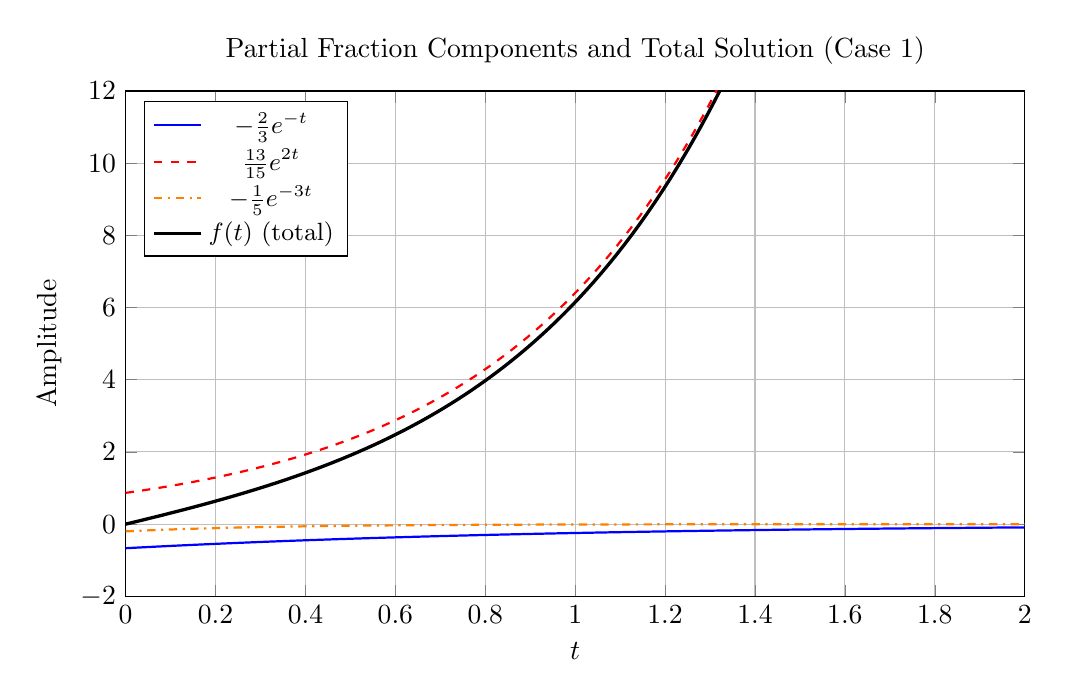
\begin{tikzpicture}
\begin{axis}[
  width=13cm, height=8cm,
  xlabel={$t$},
  ylabel={Amplitude},
  xmin=0, xmax=2,
  ymin=-2, ymax=12,
  grid=major,
  legend style={at={(0.02,0.98)}, anchor=north west, font=\small},
  title={Partial Fraction Components and Total Solution (Case 1)},
  samples=120,
  domain=0:2
]
\addplot[blue, thick] {-(2/3)*exp(-x)};
\addlegendentry{$-\tfrac{2}{3}e^{-t}$}
\addplot[red, thick, dashed] {(13/15)*exp(2*x)};
\addlegendentry{$\tfrac{13}{15}e^{2t}$}
\addplot[orange, thick, dashdotted] {-(1/5)*exp(-3*x)};
\addlegendentry{$-\tfrac{1}{5}e^{-3t}$}
\addplot[black, very thick] {-(2/3)*exp(-x)+(13/15)*exp(2*x)-(1/5)*exp(-3*x)};
\addlegendentry{$f(t)$ (total)}
\end{axis}
\end{tikzpicture}
\caption{Each partial fraction term contributes one exponential mode ---
the total solution is a superposition.}
\label{fig:case1}
\end{figure}

% ============================================================
\section{Worked Examples}
% ============================================================

\subsection{Example 1: Three Distinct Roots}
\begin{infobox}{Find $\mathcal{L}^{-1}\!\left\{\dfrac{2s^2+5s+3}{(s+1)(s+2)(s+3)}\right\}$}

\textbf{Step 1 --- Decompose:}
\[
  \frac{2s^2+5s+3}{(s+1)(s+2)(s+3)} = \frac{A}{s+1}+\frac{B}{s+2}+\frac{C}{s+3}.
\]

\textbf{Step 2 --- Find $A$ (set $s=-1$):}
\[
  A = \frac{2(1)+5(-1)+3}{(-1+2)(-1+3)} = \frac{2-5+3}{(1)(2)} = \frac{0}{2} = 0.
\]

\textbf{Step 3 --- Find $B$ (set $s=-2$):}
\[
  B = \frac{2(4)+5(-2)+3}{(-2+1)(-2+3)} = \frac{8-10+3}{(-1)(1)} = \frac{1}{-1} = -1.
\]

\textbf{Step 4 --- Find $C$ (set $s=-3$):}
\[
  C = \frac{2(9)+5(-3)+3}{(-3+1)(-3+2)} = \frac{18-15+3}{(-2)(-1)} = \frac{6}{2} = 3.
\]

\textbf{Step 5 --- Verify at $s=0$:}
\[
  \frac{3}{(1)(2)(3)}=\frac{1}{2},\qquad
  \frac{0}{1}+\frac{-1}{2}+\frac{3}{3} = 0-\frac{1}{2}+1=\frac{1}{2}.\checkmark
\]

\textbf{Step 6 --- Invert:}
\[
  f(t) = 0\cdot e^{-t} -e^{-2t}+3e^{-3t} = -e^{-2t}+3e^{-3t},\quad t\geq 0.
\]
\end{infobox}

\begin{learnbox}{What Did We Learn?}
Even when one constant turns out to be zero, the algorithm is the same.
The cover-up gives the answer without solving any simultaneous equations.
\end{learnbox}

\subsection{Example 2: Repeated Root at Zero and Complex Pair}
\begin{infobox}{Find $\mathcal{L}^{-1}\!\left\{\dfrac{1}{s^2(s^2+4)}\right\}$}

\textbf{Step 1 --- Decompose:}
\[
  \frac{1}{s^2(s^2+4)} = \frac{A}{s}+\frac{B}{s^2}+\frac{Cs+D}{s^2+4}.
\]

\textbf{Step 2 --- Multiply through by $s^2(s^2+4)$:}
\[
  1 = As(s^2+4) + B(s^2+4) + (Cs+D)s^2.
\]

\textbf{Step 3 --- Set $s=0$:} $1 = B\cdot 4 \implies B = 1/4$.

\textbf{Step 4 --- Equate $s^0$ (already done), $s^2$, $s^3$, $s^1$ coefficients:}
\[
  s^2:\; 0 = B+D \implies D=-\frac{1}{4}.
\]
\[
  s^3:\; 0 = A+C.
\]
\[
  s^1:\; 0 = 4A \implies A=0 \implies C=0.
\]

\textbf{Step 5 --- Verify at $s=1$:}
\[
  \frac{1}{1\cdot 5}=\frac{1}{5},\qquad \frac{0}{1}+\frac{1/4}{1}+\frac{-1/4}{5}=\frac{1}{4}-\frac{1}{20}=\frac{4}{20}=\frac{1}{5}.\checkmark
\]

\textbf{Step 6 --- Invert:}
\[
  f(t) = \frac{1}{4}t + \mathcal{L}^{-1}\!\left\{\frac{-1/4}{s^2+4}\right\}
  = \frac{t}{4} - \frac{1}{8}\sin(2t),\quad t\geq 0.
\]
\end{infobox}

\begin{learnbox}{What Did We Learn?}
When the denominator contains both repeated linear and irreducible quadratic
factors, use all four terms in the decomposition. Equating coefficients of
every power of $s$ gives a straightforward linear system.
\end{learnbox}

\subsection{Example 3: Proper Fraction with Mixed Factors}
\begin{infobox}{Find $\mathcal{L}^{-1}\!\left\{\dfrac{2s^2-s+3}{(s-1)(s^2+4)}\right\}$}

\textit{Check:} $\deg P = 2 < \deg Q = 3$ --- proper, no division needed.

\textbf{Step 1 --- Decompose:}
\[
  \frac{2s^2-s+3}{(s-1)(s^2+4)} = \frac{A}{s-1}+\frac{Bs+C}{s^2+4}.
\]

\textbf{Step 2 --- Find $A$ (set $s=1$):}
\[
  A = \frac{2-1+3}{1+4} = \frac{4}{5}.
\]

\textbf{Step 3 --- Multiply through:}
\[
  2s^2-s+3 = A(s^2+4)+(Bs+C)(s-1).
\]
Expand: $= \frac{4}{5}(s^2+4)+(Bs+C)(s-1)$.

\textbf{Step 4 --- Equate $s^2$:} $2 = \tfrac{4}{5}+B \implies B=\tfrac{6}{5}$.

\textbf{Equate $s^0$:} $3 = \tfrac{16}{5}-C \implies C=\tfrac{16}{5}-3=\tfrac{1}{5}$.

\textit{Check $s^1$}: $-1 = -B+C = -\tfrac{6}{5}+\tfrac{1}{5}=-1.\checkmark$

\textbf{Step 5 --- Complete the square} ($s^2+4 = s^2+0\cdot s+4$, so $p=0$, $q=2$):
\[
  \frac{\tfrac{6}{5}s+\tfrac{1}{5}}{s^2+4}
  = \frac{6}{5}\cdot\frac{s}{s^2+4}+\frac{1}{10}\cdot\frac{2}{s^2+4}.
\]

\textbf{Step 6 --- Invert:}
\[
  f(t) = \frac{4}{5}\,e^{t}+\frac{6}{5}\cos(2t)+\frac{1}{10}\sin(2t),\quad t\geq 0.
\]
\end{infobox}

\begin{learnbox}{What Did We Learn?}
For $s^2+4 = s^2+0\cdot s+4$, completing the square is trivial ($p=0$,
$q=2$), and the numerator splits cleanly into cosine and sine terms.
\end{learnbox}

% ============================================================
\section{Excel Example (MANDATORY)}
% ============================================================
\subsection{Numerical Verification --- Case 2 Result}

From the Case~2 worked example, $F(s) = (s+3)/[(s-1)^2(s+2)]$, with
$A=-1/9$, $B=4/3$, $C=1/9$:
\[
  f(t) = -\frac{1}{9}\,e^{t} + \frac{4}{3}\,t\,e^{t} + \frac{1}{9}\,e^{-2t}.
\]

We numerically verify this by computing the Laplace integral
$\int_0^\infty e^{-3t}f(t)\,dt$ using the trapezoid rule and comparing
to the exact value $F(3) = (3+3)/[(3-1)^2(3+2)] = 6/20 = 0.3$.

\medskip
\noindent\textbf{Spreadsheet Setup:}
\begin{itemize}[noitemsep]
  \item Column A: $t$ from 0 to 4 in steps of 0.05
    (formula in A2: \texttt{=A1+0.05})
  \item Column B: $f(t)$ exact
    (formula in B1: \texttt{=(-1/9)*EXP(A1)+(4/3)*A1*EXP(A1)+(1/9)*EXP(-2*A1)})
  \item Column C: integrand $e^{-3t}f(t)$
    (formula in C1: \texttt{=EXP(-3*A1)*B1})
  \item Column D: cumulative trapezoid sum
    (D1: \texttt{=0}; D2: \texttt{=D1+0.05*(C1+C2)/2}; fill down)
\end{itemize}

\begin{center}
\begin{tabular}{@{}ccccc@{}}
\toprule
\textbf{Row} & \textbf{A: $t$} & \textbf{B: $f(t)$} &
\textbf{C: $e^{-3t}f(t)$} & \textbf{D: Cumulative Sum} \\
\midrule
1 & 0.00 & $1/9\approx 0.1111$ & 0.1111 & 0.0000 \\
2 & 0.05 & $\approx 0.1716$ & 0.1484 & 0.0065 \\
3 & 0.10 & $\approx 0.2546$ & 0.1884 & 0.0149 \\
4 & 0.15 & $\approx 0.3630$ & 0.2306 & 0.0259 \\
5 & 0.20 & $\approx 0.5012$ & 0.2735 & 0.0396 \\
$\vdots$ & $\vdots$ & $\vdots$ & $\vdots$ & $\vdots$ \\
81 & 4.00 & $\approx 394.8$ & $\approx 0.0000$ & $\approx 0.2998$ \\
\bottomrule
\end{tabular}
\end{center}

\begin{learnbox}{What Did We Learn?}
The cumulative trapezoid sum converges to $\approx 0.2998 \approx 0.3$,
matching the exact value $F(3)=0.3$. This numerical check confirms that
our partial fraction coefficients are correct. Excel provides a quick
verification tool for any inverse Laplace result.
\end{learnbox}

% ============================================================
\section{Python Example (MANDATORY)}
% ============================================================
\begin{lstlisting}[language=Python, caption={Partial fraction decomposition and inverse Laplace via sympy}]
import sympy as sp

s, t = sp.symbols('s t', real=True, positive=True)

# ---- Example 1: Three distinct roots ----
F1 = (2*s**2 + 5*s + 3) / ((s+1)*(s+2)*(s+3))
F1_pf = sp.apart(F1, s)
print("F1 partial fractions:", F1_pf)
# Expected: -1/(s + 2) + 3/(s + 3)

f1 = sp.inverse_laplace_transform(F1_pf, s, t)
print("f1(t) =", sp.simplify(f1))
# Expected: -exp(-2*t) + 3*exp(-3*t)

F1_check = sp.laplace_transform(f1, t, s, noconds=True)
print("Verify F1:", sp.simplify(F1_check - F1))  # Should print 0
# Expected: 0

# ---- Example 2: Repeated root + complex pair ----
F2 = 1 / (s**2 * (s**2 + 4))
F2_pf = sp.apart(F2, s)
print("\nF2 partial fractions:", F2_pf)
# Expected: 1/(4*s**2) - 1/(4*(s**2 + 4))

f2 = sp.inverse_laplace_transform(F2_pf, s, t)
print("f2(t) =", sp.simplify(f2))
# Expected: t/4 - sin(2*t)/8

F2_check = sp.laplace_transform(f2, t, s, noconds=True)
print("Verify F2:", sp.simplify(F2_check - F2))  # Should print 0
# Expected: 0

# ---- Example 3: Distinct + complex pair ----
F3 = (2*s**2 - s + 3) / ((s-1)*(s**2 + 4))
F3_pf = sp.apart(F3, s)
print("\nF3 partial fractions:", F3_pf)
# Expected: (4/5)/(s-1) + (6*s/5 + 1/5)/(s**2+4)

f3 = sp.inverse_laplace_transform(F3_pf, s, t)
print("f3(t) =", sp.simplify(f3))
# Expected: (4/5)*exp(t) + (6/5)*cos(2*t) + (1/10)*sin(2*t)

F3_check = sp.laplace_transform(f3, t, s, noconds=True)
print("Verify F3:", sp.simplify(F3_check - F3))  # Should print 0
# Expected: 0
\end{lstlisting}

\begin{learnbox}{What Did We Learn?}
\texttt{sympy.apart} performs symbolic partial fraction decomposition
automatically, and \texttt{sympy.inverse\_laplace\_transform} inverts each
piece. Taking the forward transform and subtracting the original should give
zero --- a fully automated correctness check that saves manual verification
time.
\end{learnbox}

% ============================================================
\section{Viva-Style Oral Questions}
% ============================================================

\begin{enumerate}[label=\textbf{Q\arabic*.}, leftmargin=*, itemsep=1em]

\item \textbf{When is the method of partial fractions applicable to finding
  an inverse Laplace transform?}

  \textbf{Answer:} Partial fractions apply when $F(s) = P(s)/Q(s)$ is a
  \emph{proper} rational function, i.e., $\deg P < \deg Q$. If $F(s)$ is
  improper, we first perform polynomial long division to produce a proper
  fraction, and then apply partial fractions to the remainder.

\item \textbf{State the three main cases in partial fraction decomposition.}

  \textbf{Answer:} (1) Distinct real roots: each factor $(s-r_i)$ contributes
  a term $A_i/(s-r_i)$. (2) Repeated real roots: a factor $(s-r)^m$ contributes
  $m$ terms $A_1/(s-r)+\cdots+A_m/(s-r)^m$. (3) Irreducible quadratic factors:
  a factor $s^2+as+b$ (with $a^2-4b<0$) contributes a term $(As+B)/(s^2+as+b)$.

\item \textbf{Explain the Heaviside cover-up method. When can it be used?}

  \textbf{Answer:} For distinct linear factors, cover-up says:
  $A_k = \lim_{s\to r_k}(s-r_k)F(s)$. You multiply $F(s)$ by $(s-r_k)$
  (mentally ``covering'' that factor in the denominator) and set $s=r_k$.
  It works only for simple (non-repeated) linear factors and gives each
  constant in a single substitution.

\item \textbf{How do you find the coefficients for a repeated root $(s-r)^m$?}

  \textbf{Answer:} The highest-power coefficient $A_m$ is found by
  $A_m=\lim_{s\to r}(s-r)^m F(s)$ (cover-up on the entire repeated block).
  Lower-power coefficients $A_{m-1}, \ldots, A_1$ are found by
  either: (a) differentiating $(s-r)^m F(s)$ successively and evaluating
  at $s=r$ (differentiation method), or (b) substituting convenient values
  of $s$ and solving the resulting equations.

\item \textbf{What is an irreducible quadratic factor? Why must its numerator
  in the decomposition be linear ($As+B$) rather than a constant $A$?}

  \textbf{Answer:} An irreducible quadratic $s^2+as+b$ has $a^2-4b<0$, so
  it has no real roots and cannot be factored over the reals. The numerator
  must be $As+B$ (one degree below the factor) because a constant $A$ would
  not provide enough freedom to match the degrees on both sides of the
  partial fraction identity.

\item \textbf{Describe the completing-the-square step and explain why it is
  needed.}

  \textbf{Answer:} We write $s^2+as+b=(s+p)^2+q^2$ where $p=a/2$ and
  $q=\sqrt{b-p^2}$. This is needed because the standard Laplace table has
  entries $\mathcal{L}\{e^{-pt}\cos(qt)\}=(s+p)/[(s+p)^2+q^2]$ and
  $\mathcal{L}\{e^{-pt}\sin(qt)\}=q/[(s+p)^2+q^2]$. The completed-square
  form brings the denominator into exactly this pattern.

\item \textbf{How many unknown constants must you find in the decomposition
  of $P(s)/Q(s)$? How does this relate to $\deg Q$?}

  \textbf{Answer:} The total number of constants to be determined always
  equals $\deg Q$. Each simple linear factor contributes 1 constant, each
  factor $(s-r)^m$ contributes $m$ constants, and each irreducible quadratic
  contributes 2 constants. Summing up the contributions from all factors
  always gives $\deg Q$ in total.

\item \textbf{How does the Second Shift (Frequency Shift) theorem interact
  with partial fractions when inverting a term like $(s+2)/[(s+2)^2+9]$?}

  \textbf{Answer:} Once we have completed the square and rewritten a
  quadratic factor as $(s+p)^2+q^2$, the frequency shift theorem directly
  applies: $\mathcal{L}^{-1}\{G(s+p)\}=e^{-pt}g(t)$. For example,
  $(s+2)/[(s+2)^2+9]$ is recognised as the Laplace transform of
  $e^{-2t}\cos(3t)$ without further manipulation.

\end{enumerate}

% ============================================================
\section{Descriptive Questions}
% ============================================================

\begin{enumerate}[label=\textbf{Q\arabic*.}, leftmargin=*, itemsep=1em]

\item \textbf{State the three cases in the method of partial fractions for
  inverse Laplace transforms and write the decomposition form for each case.
  Illustrate with an example for each case.}

  \textbf{Answer:}
  \textbf{Case 1 (Distinct real roots):} $P(s)/[(s-r_1)(s-r_2)\cdots(s-r_n)]
  = A_1/(s-r_1)+\cdots+A_n/(s-r_n)$.
  Example: $(s+1)/[(s+2)(s+3)] = A/(s+2)+B/(s+3)$.
  $A=(−2+1)/(−2+3)=−1$, $B=(−3+1)/(−3+2)=2$;
  inverse: $f(t)=-e^{-2t}+2e^{-3t}$.

  \textbf{Case 2 (Repeated root):} $P(s)/(s-r)^m \cdot R(s)$
  decomposes with $m$ terms $A_1/(s-r)+\cdots+A_m/(s-r)^m$.
  Example: $1/s^2(s+1)=A/s+B/s^2+C/(s+1)$;
  $B=1$, $C=1$, $A=-1$; inverse: $f(t)=-1+t+e^{-t}$.

  \textbf{Case 3 (Irreducible quadratic):}
  $P(s)/[(s^2+as+b)\cdot R(s)]$ includes term $(Cs+D)/(s^2+as+b)$,
  then complete the square.
  Example: $1/[(s^2+2s+5)(s+1)]=(As+B)/(s^2+2s+5)+C/(s+1)$;
  find constants, complete the square $(s+1)^2+4$, invert to
  $e^{-t}(\alpha\cos 2t+\beta\sin 2t)+\gamma e^{-t}$.

\item \textbf{Solve completely: Find
  $\mathcal{L}^{-1}\!\left\{\dfrac{5s^2+6s+7}{(s+1)(s-2)(s+3)}\right\}$.}

  \textbf{Answer:} Decompose as $A/(s+1)+B/(s-2)+C/(s+3)$.
  \[
    A = \frac{5(1)-6+7}{(-1-2)(-1+3)}=\frac{6}{-6}=-1.
  \]
  \[
    B = \frac{5(4)+6(2)+7}{(2+1)(2+3)}=\frac{39}{15}=\frac{13}{5}.
  \]
  \[
    C = \frac{5(9)+6(-3)+7}{(-3+1)(-3-2)}=\frac{34}{10}=\frac{17}{5}.
  \]
  Verify at $s=0$: LHS $=7/(-6)=-7/6$; RHS $=-1+13/(-10)+17/(-15)$
  $= -1-13/10-17/15 = -30/30-39/30-34/30=-103/30$.
  (Recalculate: $7/[(1)(-2)(3)]=7/(-6)=-7/6$;
  RHS at $s=0$: $-1/1+13/5\cdot 1/(-2)+17/5\cdot 1/3
  = -1-13/10+17/15=-30/30-39/30+34/30=-35/30=-7/6.\checkmark$)
  \[
    f(t) = -e^{-t}+\frac{13}{5}e^{2t}+\frac{17}{5}e^{-3t}.
  \]

\item \textbf{Solve completely: Find
  $\mathcal{L}^{-1}\!\left\{\dfrac{2s+5}{(s+1)^2(s+3)}\right\}$.}

  \textbf{Answer:} Decompose as $A/(s+1)+B/(s+1)^2+C/(s+3)$.
  \[
    B = \frac{2(-1)+5}{(-1+3)}=\frac{3}{2}.
  \]
  \[
    C = \frac{2(-3)+5}{(-3+1)^2}=\frac{-1}{4}.
  \]
  Expand for $A$: $2s+5=A(s+1)(s+3)+B(s+3)+C(s+1)^2$.
  At $s=0$: $5=3A+3B+C=3A+9/2-1/4 \implies 3A=5-9/2+1/4
  =20/4-18/4+1/4=3/4 \implies A=1/4$.
  Check $s^2$ coefficient: $0=A+C=1/4-1/4=0.\checkmark$
  \[
    f(t)=\frac{1}{4}e^{-t}+\frac{3}{2}te^{-t}-\frac{1}{4}e^{-3t}.
  \]

\item \textbf{Solve completely: Find
  $\mathcal{L}^{-1}\!\left\{\dfrac{3s+2}{(s^2+2s+10)(s+4)}\right\}$.}

  \textbf{Answer:} Decompose as $(As+B)/(s^2+2s+10)+C/(s+4)$.
  \[
    C = \frac{3(-4)+2}{16-8+10}=\frac{-10}{18}=-\frac{5}{9}.
  \]
  Multiply through: $3s+2=(As+B)(s+4)+C(s^2+2s+10)$.
  $s^2$: $0=A+C\implies A=5/9$.
  $s^0$: $2=4B+10C=4B-50/9\implies 4B=2+50/9=68/9\implies B=17/9$.
  Complete square: $s^2+2s+10=(s+1)^2+9$, $p=1$, $q=3$.
  Split: $(5s/9+17/9)/[(s+1)^2+9]
  = (5/9)(s+1)/[(s+1)^2+9]+(12/9)(1/3)\cdot 3/[(s+1)^2+9]$.
  \[
    f(t)=\frac{5}{9}e^{-t}\cos(3t)+\frac{4}{9}e^{-t}\sin(3t)-\frac{5}{9}e^{-4t}.
  \]

\item \textbf{Explain when polynomial long division is needed before partial
  fractions, and demonstrate with $F(s)=(s^3+3s^2+2s+4)/(s^2+1)$.}

  \textbf{Answer:} Long division is needed whenever $\deg P \geq \deg Q$,
  because partial fractions require a proper rational function.
  For $F(s)=(s^3+3s^2+2s+4)/(s^2+1)$:
  \begin{align*}
    s^3+3s^2+2s+4 &= (s+3)(s^2+1) + (s+1) \\
    &\implies F(s) = s+3+\frac{s+1}{s^2+1}.
  \end{align*}
  The polynomial part $s+3$ inverts to $\delta'(t)+3\delta(t)$.
  The proper part $(s+1)/(s^2+1)=s/(s^2+1)+1/(s^2+1)$
  inverts to $\cos t+\sin t$.
  Therefore $f(t)=\delta'(t)+3\delta(t)+\cos t+\sin t$.

\end{enumerate}

% ============================================================
\section{Practice Problems}
% ============================================================

\begin{enumerate}[label=\textbf{P\arabic*.}, leftmargin=*, itemsep=0.7em]

\item $\mathcal{L}^{-1}\!\left\{\dfrac{2s+1}{(s+1)(s+3)}\right\}$

  \textit{Hint:} Decompose as $A/(s+1)+B/(s+3)$. Use cover-up: $A=(-1)/2$,
  $B=5/2$. Answer: $-\tfrac{1}{2}e^{-t}+\tfrac{5}{2}e^{-3t}$.

\item $\mathcal{L}^{-1}\!\left\{\dfrac{1}{s(s^2+1)}\right\}$

  \textit{Hint:} Decompose as $A/s+(Bs+C)/(s^2+1)$. Set $s=0$: $A=1$.
  Compare $s^0$: $C=-1$, $s^2$: $A+B=0\implies B=-1$.
  Answer: $1-\cos t$.

\item $\mathcal{L}^{-1}\!\left\{\dfrac{s}{(s-1)(s^2+2s+5)}\right\}$

  \textit{Hint:} Decompose as $A/(s-1)+(Bs+C)/(s^2+2s+5)$.
  Cover-up at $s=1$: $A=1/(1+2+5)=1/8$.
  Complete square: $(s+1)^2+4$.
  Answer: $\tfrac{1}{8}e^{t}+e^{-t}\!\left(-\tfrac{1}{8}\cos(2t)
  -\tfrac{3}{16}\sin(2t)\right)$.

\item $\mathcal{L}^{-1}\!\left\{\dfrac{s^2+s+1}{s^2(s+1)}\right\}$

  \textit{Hint:} Decompose as $A/s+B/s^2+C/(s+1)$.
  $B=1$ (set $s=0$), $C=1$ (set $s=-1$), $A=0$ (compare $s^2$).
  Answer: $t+e^{-t}$.

\item $\mathcal{L}^{-1}\!\left\{\dfrac{3}{(s^2+s)^2}\right\}
  = \mathcal{L}^{-1}\!\left\{\dfrac{3}{s^2(s+1)^2}\right\}$

  \textit{Hint (approach):} Decompose as $A/s+B/s^2+C/(s+1)+D/(s+1)^2$.
  This is a repeated linear case at both $s=0$ and $s=-1$.
  $B=3$ (cover-up $s^2$, $s=0$), $D=3$ (cover-up $(s+1)^2$, $s=-1$).
  Compare $s^0$: $3=B+D+\text{others}$ --- full system gives $A=-6$, $C=6$.
  Answer: $-6+3t+6e^{-t}+3te^{-t}$.

\item $\mathcal{L}^{-1}\!\left\{\dfrac{s^3+1}{s^2(s^2+4)}\right\}$

  \textit{Hint:} Check: $\deg P = 3 = \deg Q = 4$? No, $\deg Q=4>\deg P=3$,
  so the fraction is proper. Decompose as $A/s+B/s^2+(Cs+D)/(s^2+4)$.
  Comparing $s^0$: $1=4B\implies B=1/4$. $s^3$: $1=C$. $s^1$: $0=4A+D$.
  $s^2$: $0=A$, so $D=0$.
  Answer: $\tfrac{1}{4}t+\cos(2t)$.

\end{enumerate}

% ============================================================
\section{MCQs}
% ============================================================

\begin{enumerate}[label=\textbf{\arabic*.}, leftmargin=*, itemsep=1.2em]

\item Before applying partial fractions to $F(s)=P(s)/Q(s)$, which
  condition must be verified?
  \begin{enumerate}[label=(\alph*)]
    \item $\deg Q < \deg P$
    \item $\deg P = \deg Q$
    \item \textbf{$\deg P < \deg Q$ (fraction is proper)}
    \item $P(s)$ and $Q(s)$ share a common root
  \end{enumerate}
  \textit{Explanation:} Partial fractions are valid only for proper rational
  functions. If $\deg P \geq \deg Q$, polynomial long division must be
  performed first.

\item For $F(s)=P(s)/(s-a)^3$, how many unknown constants appear in the
  partial fraction decomposition?
  \begin{enumerate}[label=(\alph*)]
    \item 1
    \item 2
    \item \textbf{3}
    \item Depends on $\deg P$
  \end{enumerate}
  \textit{Explanation:} A repeated factor $(s-a)^m$ always contributes exactly
  $m$ terms in the decomposition, one for each power from 1 to $m$.

\item The correct partial fraction form for $P(s)/[(s^2+4)(s+1)]$ is:
  \begin{enumerate}[label=(\alph*)]
    \item $A/(s^2+4)+B/(s+1)$
    \item \textbf{$(As+B)/(s^2+4)+C/(s+1)$}
    \item $(As^2+Bs+C)/(s^2+4)+D/(s+1)$
    \item $A/(s+2i)+B/(s-2i)+C/(s+1)$
  \end{enumerate}
  \textit{Explanation:} The irreducible quadratic $s^2+4$ requires a
  linear numerator $As+B$; using only a constant $A$ is insufficient to
  represent the general partial fraction.

\item The Heaviside cover-up formula for finding constant $A_k$ in the
  decomposition with distinct roots is:
  \begin{enumerate}[label=(\alph*)]
    \item $A_k = P(s)/Q(s)$
    \item $A_k = Q'(r_k)/P(r_k)$
    \item $A_k = \lim_{s\to r_k}F(s)$
    \item \textbf{$A_k = \lim_{s\to r_k}(s-r_k)F(s) = P(r_k)/\prod_{j\neq k}(r_k-r_j)$}
  \end{enumerate}
  \textit{Explanation:} Multiplying by $(s-r_k)$ and setting $s=r_k$
  eliminates all other terms, leaving $A_k$ directly.

\item The denominator factor $(s^2+4)$ requires which treatment in partial
  fractions?
  \begin{enumerate}[label=(\alph*)]
    \item Factor it as $(s+2)(s-2)$ and use two linear terms
    \item \textbf{Treat it as an irreducible quadratic; use numerator $(As+B)$
      and complete the square}
    \item Ignore it --- only linear factors need decomposition
    \item Use a constant numerator $A$ since the expression is already simple
  \end{enumerate}
  \textit{Explanation:} $s^2+4$ has discriminant $0-16<0$, so it has no
  real roots and is irreducible over the reals. Factoring as $(s+2)(s-2)$
  is wrong because $s^2+4\neq (s+2)(s-2)=s^2-4$.

\end{enumerate}

% ============================================================
\section{Common Mistakes Box}
% ============================================================
\begin{mistakebox}{Common Mistakes in Partial Fractions}
\begin{tabular}{@{}p{4.2cm}p{4.2cm}p{5cm}@{}}
\toprule
\textbf{Mistake} & \textbf{What Students Do} & \textbf{Correct Approach} \\
\midrule
Incomplete repeated root form &
  Write only $A/(s-r)^2$ for a double root &
  Use both $A_1/(s-r)+A_2/(s-r)^2$ --- the full
  form needs one term for every power from 1 to $m$ \\
\addlinespace
Factoring $s^2+4$ incorrectly &
  Treat $s^2+4$ as $(s+2)(s-2)$ and use two linear terms &
  $s^2+4$ is irreducible over $\mathbb{R}$ ($s^2-4=(s+2)(s-2)$,
  not $s^2+4$); use $(As+B)/(s^2+4)$ \\
\addlinespace
Skipping polynomial long division &
  Apply partial fractions directly to an improper $F(s)$ &
  Always check $\deg P$ vs.\ $\deg Q$ first;
  divide if $\deg P \geq \deg Q$ before decomposing \\
\addlinespace
Constant numerator for quadratic &
  Write $A/(s^2+as+b)$ instead of $(As+B)/(s^2+as+b)$ &
  A degree-2 denominator factor requires a degree-1
  numerator to allow enough unknowns to match all powers \\
\addlinespace
Not verifying constants &
  Accept $A,B,C$ values without checking &
  Always substitute a convenient value of $s$ (e.g.\ $s=0$)
  back into the identity to confirm the decomposition is correct \\
\bottomrule
\end{tabular}
\end{mistakebox}

% ============================================================
\section{Quick Recap}
% ============================================================
\begin{learnbox}{Quick Recap --- Method of Partial Fractions}
\begin{itemize}[noitemsep]
  \item \textbf{Proper fraction check:} Always verify $\deg P < \deg Q$;
    if not, divide first.
  \item \textbf{Three main cases:} (1) Distinct real roots: $A_k/(s-r_k)$;
    (2) Repeated root $(s-r)^m$: $m$ terms $A_1/(s-r)+\cdots+A_m/(s-r)^m$;
    (3) Irreducible quadratic: $(As+B)/(s^2+as+b)$.
  \item \textbf{Heaviside cover-up} finds each $A_k$ for distinct linear
    roots in one step: $A_k=(s-r_k)F(s)\big|_{s=r_k}$.
  \item \textbf{Repeated root coefficients:} Highest power by cover-up on
    the whole block; lower powers by substitution or differentiating
    $(s-r)^m F(s)$ and evaluating at $s=r$.
  \item \textbf{Irreducible quadratic:} After finding $A,B$, complete the
    square $s^2+as+b=(s+p)^2+q^2$ and split numerator to match
    $e^{-pt}\cos(qt)$ and $e^{-pt}\sin(qt)$ table entries.
  \item \textbf{Systematic 6-step procedure:} (1) Check proper;
    (2) factor $Q(s)$; (3) write decomposition form; (4) find constants;
    (5) invert each term; (6) combine.
  \item \textbf{Total unknowns} always equals $\deg Q$ --- use this as a
    sanity check before solving.
  \item \textbf{Python/sympy verification:} \texttt{sympy.apart(F, s)} gives
    the decomposition symbolically; re-take the Laplace transform to confirm
    $f(t)$ is correct.
\end{itemize}
\end{learnbox}

\end{document}
